\textbf{\underline{OZ 4 - De wet van Ampère en de wet van Biot-Savart - Oefening 3:}}
\vspace{0.5cm}

\begin{minipage}{0.7\textwidth}
    \vspace{-2cm}
    Een niet-geleidende schijf van straal $R$ draagt een uniform verdeelde lading $Q$. De schijf wordt rondgedraaid met een hoeksnelheid $\omega$ rond een as loodrecht op het vlak
    van de schijf en door het centrum van de schijf.
\end{minipage}
\begin{minipage}{0.26\textwidth}
    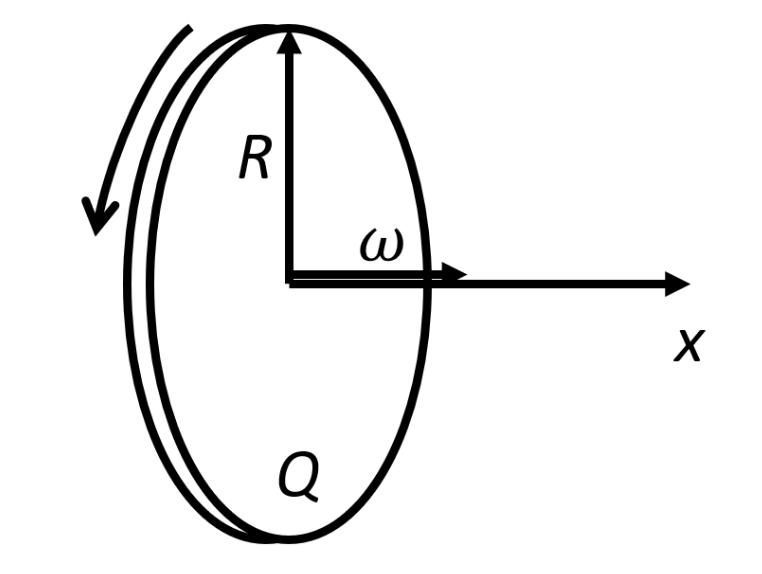
\includegraphics[scale = 0.3]{oz04/resources/Oz4Oef3.png}
\end{minipage}

\vspace{-2cm}

% \begin{description}[labelwidth=1.5cm, leftmargin=!]
%     \item[Geg. :]  
%     \item[Gevr. :] 
%     \item[Opl. :]  
% \end{description}

\begin{enumerate}[(a)]
    \item Bepaal het magnetische dipoolmoment van de schijf.
    \item Bepaal het magnetische veld op de rotatie-as op een afstand $x$ 
          \\ van het centrum van de schijf.
    \item Als $x >> R$ reduceert de uitkomst van (b) dan naar de formule
          \\ voor een magnetische dipool?
\end{enumerate}

\begin{enumerate}[(a)]
    \item 
        \begin{description}[labelwidth=1.5cm, leftmargin=!]
            \item[Geg. :]  $R$, $Q$, $\omega$
            \item[Gevr. :] $\Vec{\mu}$ ?
            \item[Opl. :]  
                         We stellen de formule van het infinitesimale oppervlakte op
                         \begin{align}
                             dA &= 2\pi rdr \nonumber \\ 
                            \intertext{waaruit we de formule voor de infinitesimale lading kunnen afleiden}
                             dq &= \dfrac{Q}{A} dA \nonumber \\ 
                                &= \dfrac{Q}{R^2}2rdr \\
                            \intertext{We weten de formule van de periode van de cirkelbeweging}
                            T &= \dfrac{2\pi}{\omega}  \\ 
                            \intertext{Uit (1) en (2) vinden we}
                             dI &= \dfrac{dq}{dt} \nonumber \\ 
                                &= \dfrac{dq}{T} \nonumber \\ 
                                &= \dfrac{Q\omega}{R^2\pi}rdr \nonumber \\
                                % &= \omega r^2dr \nonumber \\
                            \intertext{waaruit we de infinitesimale magnetisch dipoolmoment kunnen halen}
                           d\mu &= dI(\pi r^2) \nonumber \\ 
                                % &= (\omega cr^2dr)(\pi r^2) \\ 
                                &= \dfrac{Q\omega}{R^2}r^3 dr \nonumber
                            \intertext{en dus het magnetisch dipoolmoment}
                            \mu &= \int_0^R d\mu \nonumber \\ 
                                &= \dfrac{Q\omega}{R^2} \int_0^R r^3 dr \nonumber \\ 
                                &= \dfrac{Q \omega R^2}{4} \nonumber \\
                            \intertext{Vectorieel wordt dit:}
                            \Vec{\mu} &= \dfrac{Q \omega R^2}{4} \ (\hat{i}) \nonumber
                         \end{align}
        \end{description}
        \newpage
        
    \item 
        \begin{description}[labelwidth=1.5cm, leftmargin=!]
            \item[Geg. :]  $R$, $Q$, $\omega$
            \item[Gevr. :] $B_x$ ?
            \item[Opl. :]  
                        We berekenen eerst het magnetisch veld in het centrum van een cirkel met straal $r$
                        \begin{align*}
                            B_{\text{cirkel},x} 
                                &= \frac{\mu_0I}{4\pi} \int \frac{d\ell}{r^2 + x^2} \sin(\phi) \\
                                &= \frac{\mu_0I}{4\pi} \int \frac{r}{r^2 + x^2} \sin(\phi) d\theta \\
                                &= \frac{\mu_0I}{4\pi}  \int \frac{r}{r^2 + x^2} \frac{r}{\sqrt{r^2+x^2}} d\theta \\
                                &= \frac{\mu_0 Q\omega r}{4\pi^2 R^2} \frac{r}{r^2 + x^2} \frac{r}{\sqrt{r^2+x^2}} \int_0^{2\pi} d\theta \\
                                &= \frac{\mu_0 Q\omega r^3}{2\pi R^2(r^2 + r^2)^{\tfrac{3}{2}}} \\
                                \intertext{
                                    waarbij $I = \frac{Q\omega}{R^2\pi}r$, wat we berekent hadden in (a).  Een schijf bestaat uit infinitesimale cirkels en dus integreren we over bovenstaande formule om het magnetisch veld door de schijf te verkrijgen
                                }
                                B_{\text{schijf},x} 
                                &= \int dB_{\text{cirkel},x} \\
                                % &= \int \frac{\mu_0dI}{2\pi} \frac{r^2}{(r^2 + x^2)^{\tfrac{3}{2}}} \\
                                &= \int \frac{\mu_0 Q\omega r^3}{2\pi R^2(r^2 + r^2)^{\tfrac{3}{2}}}  dr \\
                                % &= \int \frac{\mu_0}{2\pi} \frac{Q\omega r}{\pi R^2} \frac{r^2}{(r^2 + x^2)^{\tfrac{3}{2}}} dr \\
                                &= \frac{\mu_0Q\omega}{2\pi R^2} \int_0^R \frac{r^3}{(r^2 + x^2)^{\tfrac{3}{2}}} \\
                                &= \frac{\mu_0Q\omega}{2\pi R^2}\left(\sqrt{x^2+R^2} + \frac{x^2}{\sqrt{x^2+R^2}} - 2x\right) 
                        \end{align*}
        \end{description}
        
    \item 
        \begin{description}[labelwidth=1.5cm, leftmargin=!]
            \item[Geg. :]  $x >> R$, $ B_{\text{dipool}} \approx \frac{\mu_0}{2\pi} \frac{\mu}{x^3}$
            \item[Gevr. :] $ B_{\text{schijf},x} \approx B_{\text{dipool}}$ ?
            \item[Opl. :]  
            We beginnen door $B_{\text{schijf},x}$ te herschrijven
            \begin{align*}
                B_{\text{schijf},x}
                    &= \frac{\mu_0Q\omega}{2\pi R^2}\left(\sqrt{x^2+R^2} + \frac{x^2}{\sqrt{x^2+R^2}} - 2x\right) \\
                    &= \frac{\mu_0Q\omega x}{2\pi R^2}\left(\sqrt{1+\frac{R^2}{x^2}} + \frac{1}{\sqrt{1+\frac{R^2}{x^2}}} - 2\right) 
            \end{align*}
            We nemen de derde-orde taylorreeks van $\sqrt{1+y^2}$ en $(\sqrt{1+y^2})^{-1}$ 
            \begin{align*}
                \sqrt{1+y^2} 
                    &= 1 + \frac{1}{2}y - \frac{1}{8}y^2 \\
                \frac{1}{\sqrt{1+y^2}} 
                    &=  1 - \frac{1}{2}y + \frac{3}{8}y^2 \\
            \end{align*}
            waaruit volgt
            \begin{equation*}
                 B_{\text{schijf},x} = \frac{\mu_0Q\omega R^2}{8\pi x^3} = \frac{\mu_0}{2\pi} \frac{\mu}{x^3} \approx B_{\text{dipool}}                  
            \end{equation*}
        \end{description}
\end{enumerate}


\vspace{1cm}